\section{Baza danych}

Dane przechowywane są w relacyjnej bazie danych \textbf{PostgreSQL}, w ramach schematu \texttt{public} bazy \texttt{javabase}. System korzysta z następujących tabel:

\begin{itemize}
    \item \texttt{zajecia} – główna tabela przechowująca dane o wszystkich zajęciach:
    \begin{itemize}
        \item \texttt{id}, \texttt{typ}, \texttt{kierunek}, \texttt{przedmiot}, \texttt{prowadzacy}, \texttt{sala}, \texttt{dzien}, \texttt{godzina}, \texttt{grupa1}, \texttt{grupa2}.
    \end{itemize}

    \item \texttt{projekty} – zawiera przypisanie dwóch grup do zajęć typu \texttt{Projekt}:
    \begin{itemize}
        \item \texttt{zajecia\_id}, \texttt{grupa1}, \texttt{grupa2}.
    \end{itemize}

    \item \texttt{laboratoria} – przechowuje numer grupy przypisanej do zajęć typu \texttt{Laboratorium}:
    \begin{itemize}
        \item \texttt{zajecia\_id}, \texttt{nr\_grupy}.
    \end{itemize}

    \item \texttt{uzytkownicy} – tabela logowania przechowująca dane uwierzytelniające użytkowników:
    \begin{itemize}
        \item \texttt{id}, \texttt{login}, \texttt{haslo}.
    \end{itemize}
\end{itemize}

Tabele są powiązane logicznie przez kolumnę \texttt{zajecia\_id}, a dane zabezpieczone są poprzez ograniczenia integralności oraz indeksy. Struktura została zaprojektowana tak, aby umożliwiać wygodne wykonywanie operacji CRUD i filtrowania.

\section{Diagram Baza Danych}

\begin{figure}[H]
    \centering
    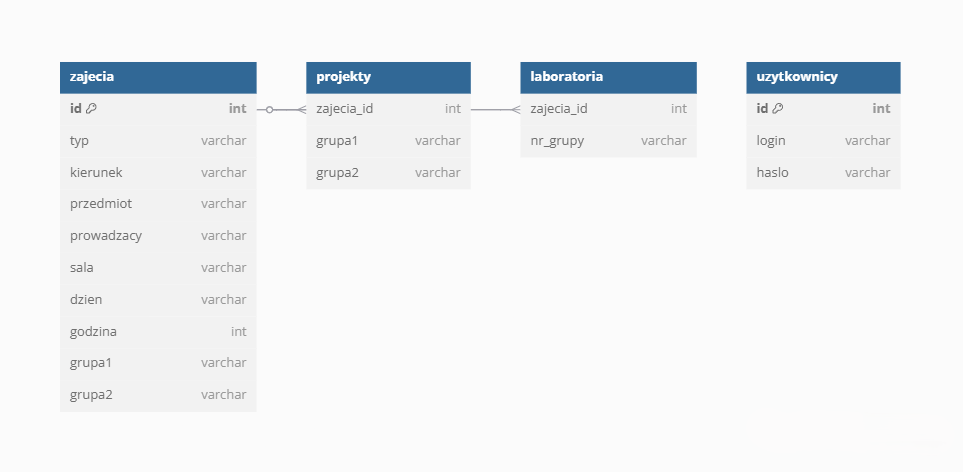
\includegraphics[width=0.85\textwidth]{figures/diagramDB.png}
    \caption{Diagram relacyjny bazy danych systemu}
    \label{fig:diagram-db}
\end{figure}